\begin{figure}[h!] 
	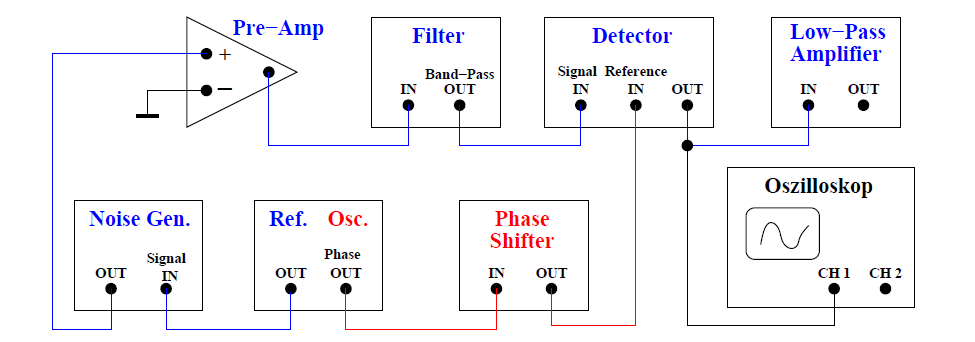
\includegraphics[width =  \textwidth]{Versuch.png}
\caption[Aufbau des ersten und zweiten versuchteils]{Aufbau des ersten und zweiten Versuchsteils \footnotemark}
	\label{versuch}
\end{figure}	
\footnotetext{entnommen aus der Versuchsanleitung V303}

In Abbildung \ref{versuch} ist ein schematischer Aufbau des Lock-In-Verstärkerts dargestellt.  \\
Bevor der eigentliche Versuch startet, ist die erste Aufgabe die Ausgangssignale (Reference/Oscilator) abzugreifen und mit einem Oszilloskop zu untersuchen. Beide Signale haben die gleiche Frequenz, die  \SI{1}{\kilo\hertz} gewählt wird. Das Referenzsignal hat eine unveränderliche Amplitude von \SI{30}{\volt}. Die Amplitude des Ausgangssignals soll klein, möglichst auf \SI{10}{\milli\volt} eingestellt werden. \\
In ersten Versuchsteil wird das reine Ausgangssignal ohne ein Rauschsignal betrachtet. Das Signal gelangt durch einen Verstärker in den Bandpass, um dann mit dem Referenzsignal vermischt zu werden (Detector). Die Phase des Referenzsignals kann vorher verschoben werden (Phase Shifter). Das Produkt beider Signale ist auf einem digitalen Oszilloskop zu sehen. Dieses Signal wird im Tiefpass integriert (Low-Pass-Filter), um $U_0$ zu erhalten. Die Oszilloskopbilder und die Spannungswerte $U_0$ werden für verschiedene Phasendifferenzen bestimmt. \\
Im zweiten Versuchsteil wird das Ausgangssignal von einem Rauschen überlagert (Noise Generator). Der restliche Aufbau bleibt unverändert und es werden ebenfalls Werte und Bilder für verschiedene Phasendifferenzen genommen. \\
\begin{figure}[h!]
	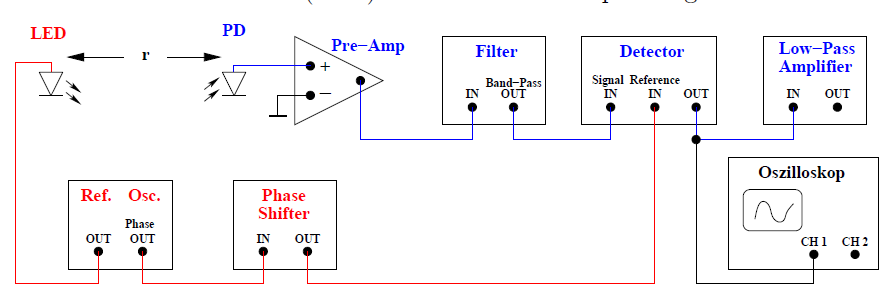
\includegraphics[width = \textwidth]{Lampe.png}
	\caption{Messung der Lichtintensität einer LED\protect\footnotemark}
	\label{lampe}
\end{figure}	
\footnotetext{entnommen aus der Versuchsanleitung V303}
	
Zum Schluss soll die Lichtintensität einer blinkenden LED in Abhängigkeit des Abstandes zum Messgerät, einer Photodiode, gemessen werden. Je weiter die Photodiode von der LED entfernt ist, desto größer ist das Hintergrundrauschen durch einfallendes Licht aus der Umgebung. Es soll der Abstand $r_\text{max}$ bestimmt werden, bei dem das Signal der LED nicht mehr erkennbar ist. Dazu wird der vorherige Aufbau leicht verändert, wie in Abbildung \ref{lampe} gezeigt ist. Die LED wird an die Rechteckspannung angeschlossen. Das Referenzsignal wird mit dem Signal der LED mit Hilfe des Phasenverschiebers  mit dem der LED in Phase gebracht. Das im Photodetektor registrierte Signal wird beliebig verstärkt (Pre-Amplifier).
